\documentclass[10pt]{beamer}
\usetheme{Madrid}
\usepackage[utf8]{inputenc}
\usepackage[english]{babel}
\usepackage{amsmath}
\usepackage{amsfonts}
\usepackage{amssymb}
\usepackage{graphicx}
\usepackage{multicol}
\usepackage{pifont}
\usepackage{listings}
 
 
\usepackage{color}
 
\definecolor{dkgreen}{rgb}{0,0.6,0}
\definecolor{gray}{rgb}{0.5,0.5,0.5}
\definecolor{mauve}{rgb}{0.58,0,0.82}
 
\lstset{ %
  language=C,                
  basicstyle=\footnotesize,     
  numbers=left,               
  numberstyle=\tiny\color{gray},
  stepnumber=1,                                       
  numbersep=4pt,                 
  backgroundcolor=\color{white},  
  showspaces=false,             
  showstringspaces=false,         
  showtabs=false,                 
  frame=single,                   
  rulecolor=\color{black},       
  tabsize=4,                   
  captionpos=b,        
  breaklines=true,             
  breakatwhitespace=false,       
  title=\lstname,                                                  
  keywordstyle=\color{blue},          
  commentstyle=\color{dkgreen},    
  stringstyle=\color{mauve},       
  escapeinside={\%*}{*)},        
  morekeywords={*,...}              
}




%\author{}
\title{MODULE 5 Advanced Topics}
%\setbeamercovered{transparent} 
%\setbeamertemplate{navigation symbols}{} 
\logo{
\includegraphics[scale=0.2]{aucalogo.png}} 
\institute[]{ADVENTIST UNIVERSITY OF CENTRAL AFRICA \\ FACULTY OF INFORMATION TECHNOLOGY
\\ Course: \textbf{Mobile Programming\\ INSY 429 \\GROUP IV}} 
\date{\today} 

%\subject{} 
\begin{document}

\begin{frame}

\titlepage

\end{frame}

\begin{frame}{Group Members}
\textbf{Group IV:}

\begin{enumerate}
\begin{multicols}{2}
\item RUKUNDO Justin 23456
\item NZEYIMANA Yvon Miracle 23707
\item MUKARWAKA UWASE Mireille 23621
\item Iradukunda Divine 23663
\item ABAYO Florence 23413
\item NIYIRERA Jacqueline 24103
\item kengne klinsman 24042
\item Rafiki Didier 22709
\item Rocky Kayitare 24353
\item Kalisa Sangwa Kelly 23652
\item Ntore Ntwari Rumenera 24438
\item Warda Umutoni  20500
\item Igiraneza Michel 23674
\item Ali Mohamadene Haroun 24315
\item Mucyo Herve 23745
\item Emmanuel MANZI 24031
\item Rwego Muhoza Alain Patrick 23738
\item Niyokwizera Jean de Dieu 21681
\item SHYAKA Dieu-Merci R.  24232
\item Iradukunda Lea 23279
\item IZERE Didier 23423 
\item MUGABO Andr\'e 25337

\end{multicols}
\end{enumerate}
\end{frame}

\begin{frame}{Table of Contents}
%\begin{multicols}{2}
\tableofcontents
%\end{multicols}
\end{frame}
\begin{frame}{INTRODUCTION}
\section{Introduction}
\textbf{Introduction}\\
This presentation will focus on module 5 entitled \textbf{Advanced Topics} of our course  \textbf{Mobile Programming INSY 429} that has as objective of empowering a students with the following   topics :
\begin{block}{Upon completion of the module, the student should acquire the capacity to:}
\begin{enumerate}
\item[\ding{242}] Implementing authentication and user management
\item[\ding{242}] Integrating with device features (e.g., Camera, Geolocation, Sensors) 
\item[\ding{242}] Push notifications and background tasks
\item[\ding{242}] Performance optimization techniques
\item[\ding{242}] Testing and debugging React Native applications

 
\end{enumerate}
\end{block}
Now let's see one by one of the above topics

\end{frame}

\begin{frame}{Implementation of authentication and user management}
\section{Implementation of authentication and user management}
\begin{block}{Authentication}
\textbf{Authentication} plays a vital role in modern applications and services by enabling them to identify the user and regulate their authorized actions.
\begin{enumerate}
\item[\ding{230}]React Native authentication refers to the process of verifying the identity of a user in a React Native app.
\item[\ding{230}]This is typically done by asking the user to provide their login credentials, such as a username and password.
\item[\ding{230}] Then checking those credentials against a database of authorized users.




\end{enumerate} 
\end{block}

\end{frame}

\begin{frame}{Implementation of authentication and user management}
\begin{block}{OAuth 2.0 authorization framework}
React Native authentication is commonly implemented with OAuth 2.0
\begin{enumerate}
\item[\ding{230}]This allows users to sign in via popular third-party services such as Google, Facebook, or Twitter.
\item[\ding{230}]There are several libraries you can use to implement authentication in React Native-we'll cover three of them in this presentation.
\begin{enumerate}
\item React Native App Auth
\item React Navigation
\item React Native OAuth
\end{enumerate}
\end{enumerate}

\end{block}

\end{frame}

\begin{frame}{Why is React Native authentication important?}
\subsection{Why is React Native authentication important?}
\begin{enumerate}
\item[\ding{230}]React Native authentication is critical because it provides a secure way for users to access protected resources in a React Native app.
\item[\ding{230}]Without proper user authentication, anyone could access sensitive information or perform actions that they should not be able to. 
\begin{block}{React Native authentication is important for:}
\begin{enumerate}
\item[\ding{242}]Protecting sensitive data.
\item[\ding{242}]Enhancing security.
\item[\ding{242}]Improving user experience.
\item[\ding{242}]Supporting compliance.
\end{enumerate}
\end{block}
\end{enumerate}
\end{frame}

\begin{frame}{Implementing React Native authentication with OAuth2}
\subsection{Implementing React Native authentication with OAuth2}
\begin{block}{OAuth2}
\begin{enumerate}
\item[\ding{230}]OAuth2 is an open standard for authorization that's widely used to allow users to grant access to resources without sharing their credentials.
\item[\ding{230}]In the context of React Native authentication,
\item[\ding{230}]OAuth2 is commonly used to allow a user to sign in to an application using their existing credentials from a third-party service, such as Google, Facebook, or Twitter.
\end{enumerate}

\end{block}
\begin{center}
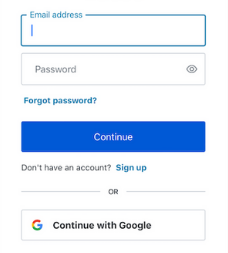
\includegraphics[scale=.2]{2.png}
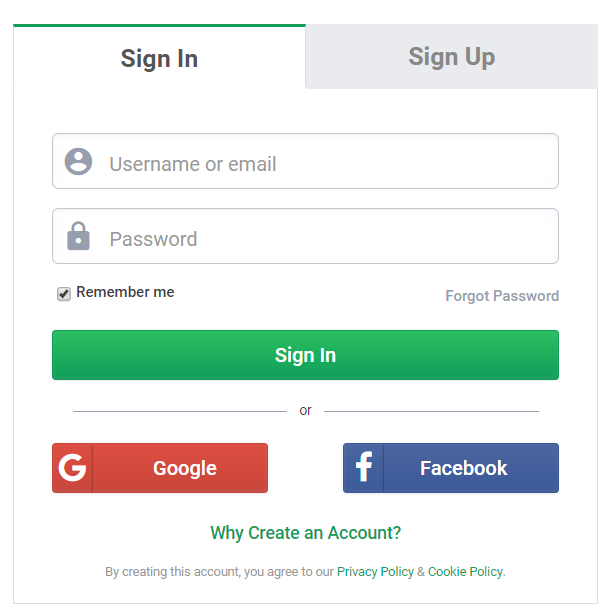
\includegraphics[scale=.2]{1.png}
\end{center}

\end{frame}

\begin{frame}{Implementing React Native authentication with OAuth2}
\begin{block}{OAuth2}
\begin{enumerate}
\item[\ding{230}]A common flow for OAuth2 in a React Native application is for the user to click a "Sign in with X" button, which then redirects them to the third-party service's login page.
\item[\ding{230}] Once the user has successfully logged in to the third-party service, they are redirected back to the React Native application, where they grant permission for the application to access their resources.


\end{enumerate}

\end{block}

\end{frame}

\begin{frame}{Implementing React Native authentication with OAuth2}
\begin{block}{OAuth2}
\begin{enumerate}
\item[\ding{230}] Redirects are an important part of the OAuth2 flow in React Native applications. The redirects are used to redirect the user to the third-party service's login page, and then back to the React Native application after the user has successfully logged in.
\item[\ding{230}] These redirects are typically implemented using the \textbf{WebView component}  in React Native, which is used to display web pages within the mobile application.
\end{enumerate}
\end{block}
\end{frame}

\begin{frame}{What is Proof of Key Code Exchange or PKCE?}
\subsection{What is Proof of Key Code Exchange or PKCE?}
\begin{block}{Proof of Key Code Exchange, or PKCE}
\begin{enumerate}
\item[\ding{230}]Proof of Key Code Exchange, or PKCE, is an extension to the OAuth2 authorization code flow that provides additional security for public client applications.
\item[\ding{230}] In the standard OAuth2 authorization code flow, an authorization code is exchanged for an access token. This can create security vulnerabilities, as a malicious actor could intercept the authorization code and use it to obtain an access token for the user's resources. 
\item[\ding{230}] PKCE solves this problem by adding an extra step to the authorization code flow, where a code verifier is generated and passed along with the authorization code. The code verifier is then used to verify the authorization code when it is exchanged for an access token, providing an additional layer of security.


\end{enumerate}

\end{block}

\end{frame}

\begin{frame}{React Native authentication libraries }
\subsection{React Native authentication libraries}
\subsection{React Native authentication libraries}
\begin{block}{React Native authentication libraries}
There is a variety of libraries you can use to implement authentication in your React Native apps. The three discussed here are only a few of the possible options-there are many more libraries you could use to implement authentication in React.
\end{block}

\end{frame}

\begin{frame}{React Native authentication libraries}
\subsubsection{React Native App Auth}
\begin{block}{React Native App Auth}
\begin{enumerate}
\item[\ding{242}]\textbf{React Native App Auth} is an open-source library for implementing authentication in React Native apps using OAuth 2.0 and OpenID Connect. It provides a set of tools and APIs for interacting with OAuth 2.0 and OpenID Connect-compliant identity providers, such as Google, Facebook, and Microsoft, to authenticate users.
\item[\ding{242}]React Native App Auth supports both Android and iOS platforms and can be easily integrated into a React Native app to handle authentication tasks, such as user login and logout, securely storing authentication tokens, and refreshing access tokens.



\end{enumerate}
\end{block}
\end{frame}

\begin{frame}{React Native authentication libraries}
\begin{block}{React Native App Auth}
\begin{enumerate}
\item[\ding{242}]The library abstracts the underlying authentication protocol details, making it easier for developers to implement authentication in their apps without having to deal with the complexity of the underlying protocols.
\end{enumerate}
\end{block}
\begin{block}{React Navigation}
\subsubsection{React Navigation}
\begin{enumerate}
\item[\ding{242}]\textbf{React Navigation} is a popular library for navigation in React Native apps. It provides tools and APIs for navigation between screens, handling navigation history, and configuring the navigation header. 
\item[\ding{242}]React Navigation can be used in combination with a separate authentication library to implement authentication in a React Native app by controlling the navigation flow based on the authentication state.
\end{enumerate}

\end{block}
\end{frame}

\begin{frame}{React Native authentication libraries}
\begin{block}{React Native OAuth}
\subsubsection{React Native OAuth}
\begin{enumerate}
\item[\ding{242}]React Native OAuth is a library for adding OAuth authentication to React Native apps. With React Native OAuth, developers can add OAuth authentication to their apps and interact with OAuth-compliant identity providers, such as Google, Facebook, and Microsoft, to authenticate users. The library provides a set of APIs and tools for handling common OAuth tasks, such as obtaining and refreshing access tokens, securely storing tokens, and handling token expiration.
\item[\ding{242}]React Native OAuth supports both Android and iOS platforms and can be easily integrated into a React Native app to handle authentication tasks.
\end{enumerate}
\end{block}
\end{frame}

\begin{frame}{React Native authentication example }
\begin{block}{Authentication Example}
Here's an example of how to use the React Native App Auth library to implement OAuth 2.0 authentication in a React Native app.\\
First, install the React Native App Auth library:
\begin{center}

\includegraphics[scale=.5]{3.png}
\end{center}
Import the React Native App Auth module into your React Native app:
\lstinputlisting[language=Java]{Auth.js}
\end{block}
Add a function to handle the authorization flow:
\end{frame}

\begin{frame}{React Native authentication example}
\begin{block}{Authentication Example}

\lstinputlisting[language=Java]{handleAuthorize.js}
\end{block}

\end{frame}
\begin{frame}{React Native authentication example}
\begin{block}{Authentication Example}
Add a function to handle sign-out:
\lstinputlisting[language=Java]{handleSignOut.js}
Use the above functions in your React Native app to authorize and sign out users.

\end{block}

\end{frame}



















\end{document}